\documentclass{article}
\usepackage[minionint,mathlf,textlf]{MinionPro} % To gussy up a bit
\usepackage[margin=1in]{geometry}
\usepackage{graphicx} % For .eps inclusion
%\usepackage{indentfirst} % Controls indentation
\usepackage[compact]{titlesec} % For regulating spacing before section titles
\usepackage{adjustbox} % For vertically-aligned side-by-side minipages
\usepackage{array, mathrsfs, mathrsfs, mhchem, amsmath} % For centering of tabulars with text-wrapping columns
\usepackage{hyperref, chemfig}
\usepackage{subfigure}
\usepackage[autolinebreaks,framed,numbered]{mcode}
\newcommand{\Lapl}{\mathscr{L}}

\pagenumbering{gobble} 
\setlength\parindent{0 cm}
\begin{document}
\large

\section*{Introduction to self-assembly}

Self-assembly is the process by which components join to form a desired structure without the help of an external agent. For example, a protein formed from subunits which remain bound together after randomly colliding has undergone self-assembly, whereas a messenger RNA produced through joining of free nucleotides by a proteinaceous polymerase has not. If all or even most complex structures in biology required an agent dedicated to their own construction, then an enormous number of components would be necessary: it is therefore likely that many biological structures manage to construct themselves through component ``design" that exploits the laws of physics and chemistry. Self-assembly is also of particular interest for the evolution of life, a condition in which other organic agents cannot be invoked to aid in replication. Producing building blocks which self-assemble is a simple strategy for self-replication, one of the fundamental processes of life.

\section*{Self-assembly of virions}

Consider the dilemma faced by a virus which must encapsulate its genome and release it from a host cell as an infectious virion. Every base pair in the viral genome (assuming that it is double-stranded) weighs around 600 Da, and it takes three such base pairs to encode a single 100-Da amino acid in the viral proteome, yet many viruses produce a proteinaceous capsid that completely encloses the genome. All of this is achieved despite many negative charges on the phosphodiester backbone of DNA that tend to impede the genome's compression through electrostatic repulsion. The situation merits a detailed analysis since many gene therapy and bioengineering applications require delivering synthetic sequences via virion, and knowing the limitations on size and sequence would be helpful for developing new vectors.\\

Key strategies of which you may be aware include producing a capsid from many copies of a small number of proteins by taking advantage of symmetry; positively-charged protein domains that partially neutralize the viral genome's charge through associations with the backbone; and encoding proteins in overlapping open reading frames to minimize the genome's size. Even with these clever approaches, there are still some serious challenges. The simian vacuolating virus SV40, for example, is an icosahedral virus with no plasma membrane envelope, i.e., the protein capsid is the only structure maintaining integrity of the virion. The capsid comprises three hundred and sixty copies of the same protein, arranged into 72 pentamers. Some of these pentamers (at each vertex of the icosahedron) have five neighbors; others, six.

\begin{center}
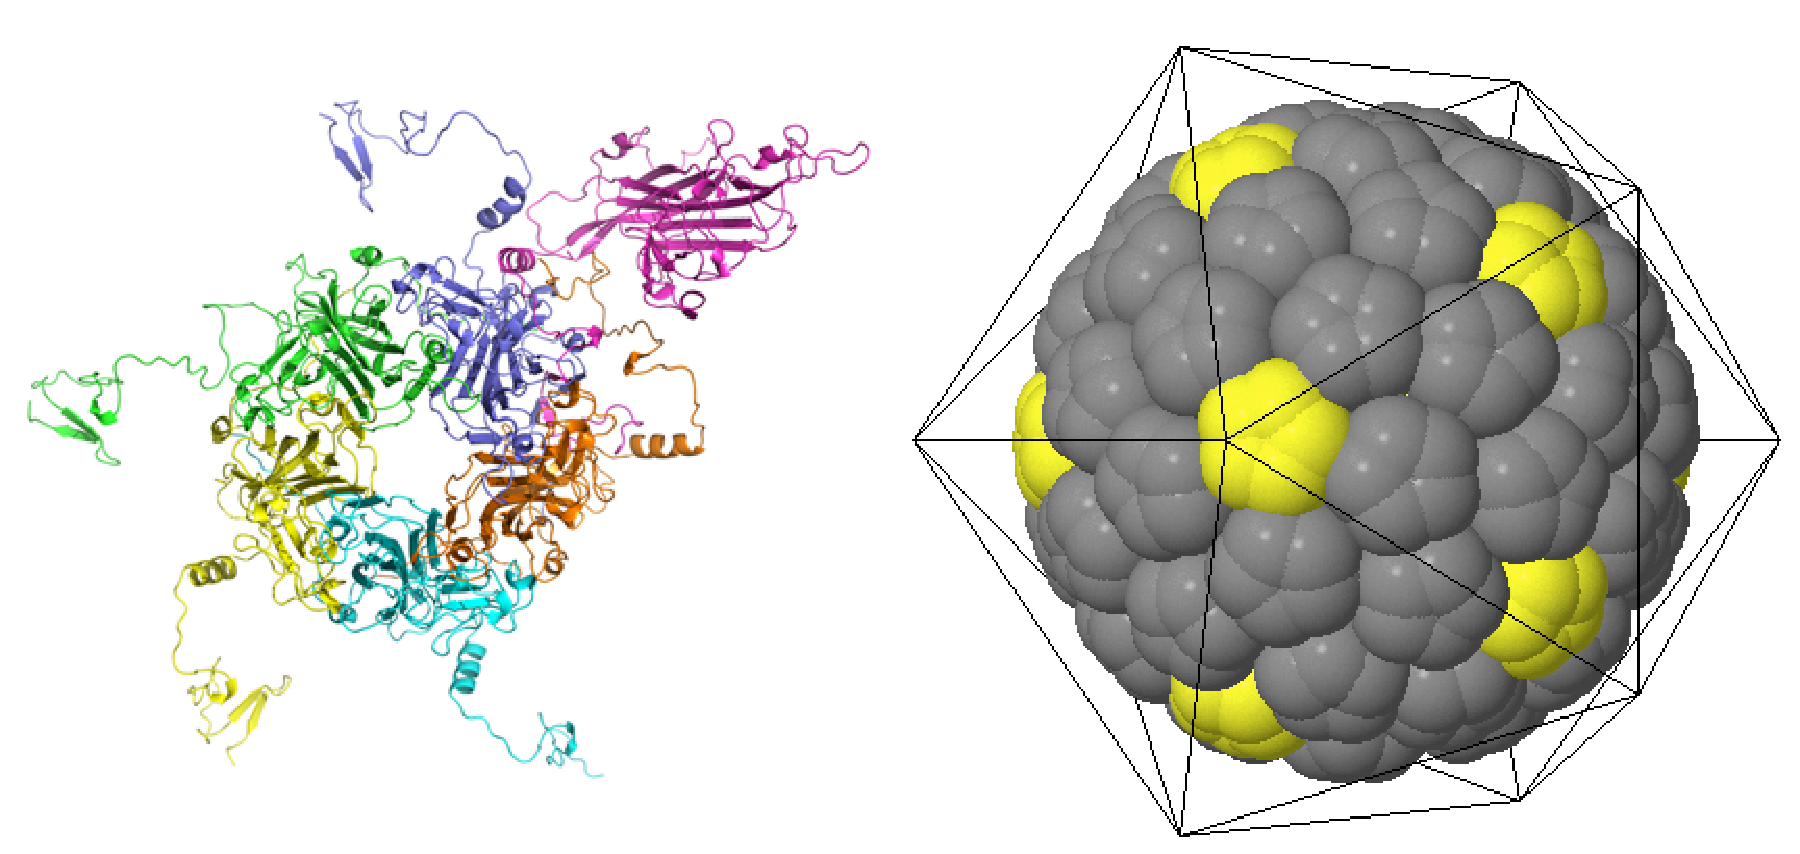
\includegraphics[width=0.7\textwidth]{sv40.pdf}
\end{center}

Nonspecific interactions between host cell proteins and even a small fraction of these three hundred and sixty virion proteins could prevent the capsid from properly forming. A typical theme in viral capsid formation is that single subunits assemble into multi-subunit complexes (equivalent in SV40 to the pentamers), which in turn can form small groups or sheets that interact to complete the capsid. Each of these assembly steps creates a larger interface between interacting units that likely is stabilizing only if all units are correctly assembled. In this way properly-assembled pentamers are preferentially incorporated into groups/sheets and properly-assembled groups/sheets are incorporated into the capsid.\\

Another major issue in assembly is that a copy of the viral genome must be incorporated inside of the capsid when it assembles. Some viral genomes contain packaging sequences that help the capsid assemble around the genome through specific binding, but it appears in many cases that only size (folded or otherwise) and charge determine the likelihood that a nucleic acid will be incorporated. Though capsid proteins often have positive charge on their interior surfaces as mentioned above, it is rarely enough to balance the negative charge of the nucleic acid contained within the capsid.

\begin{center}
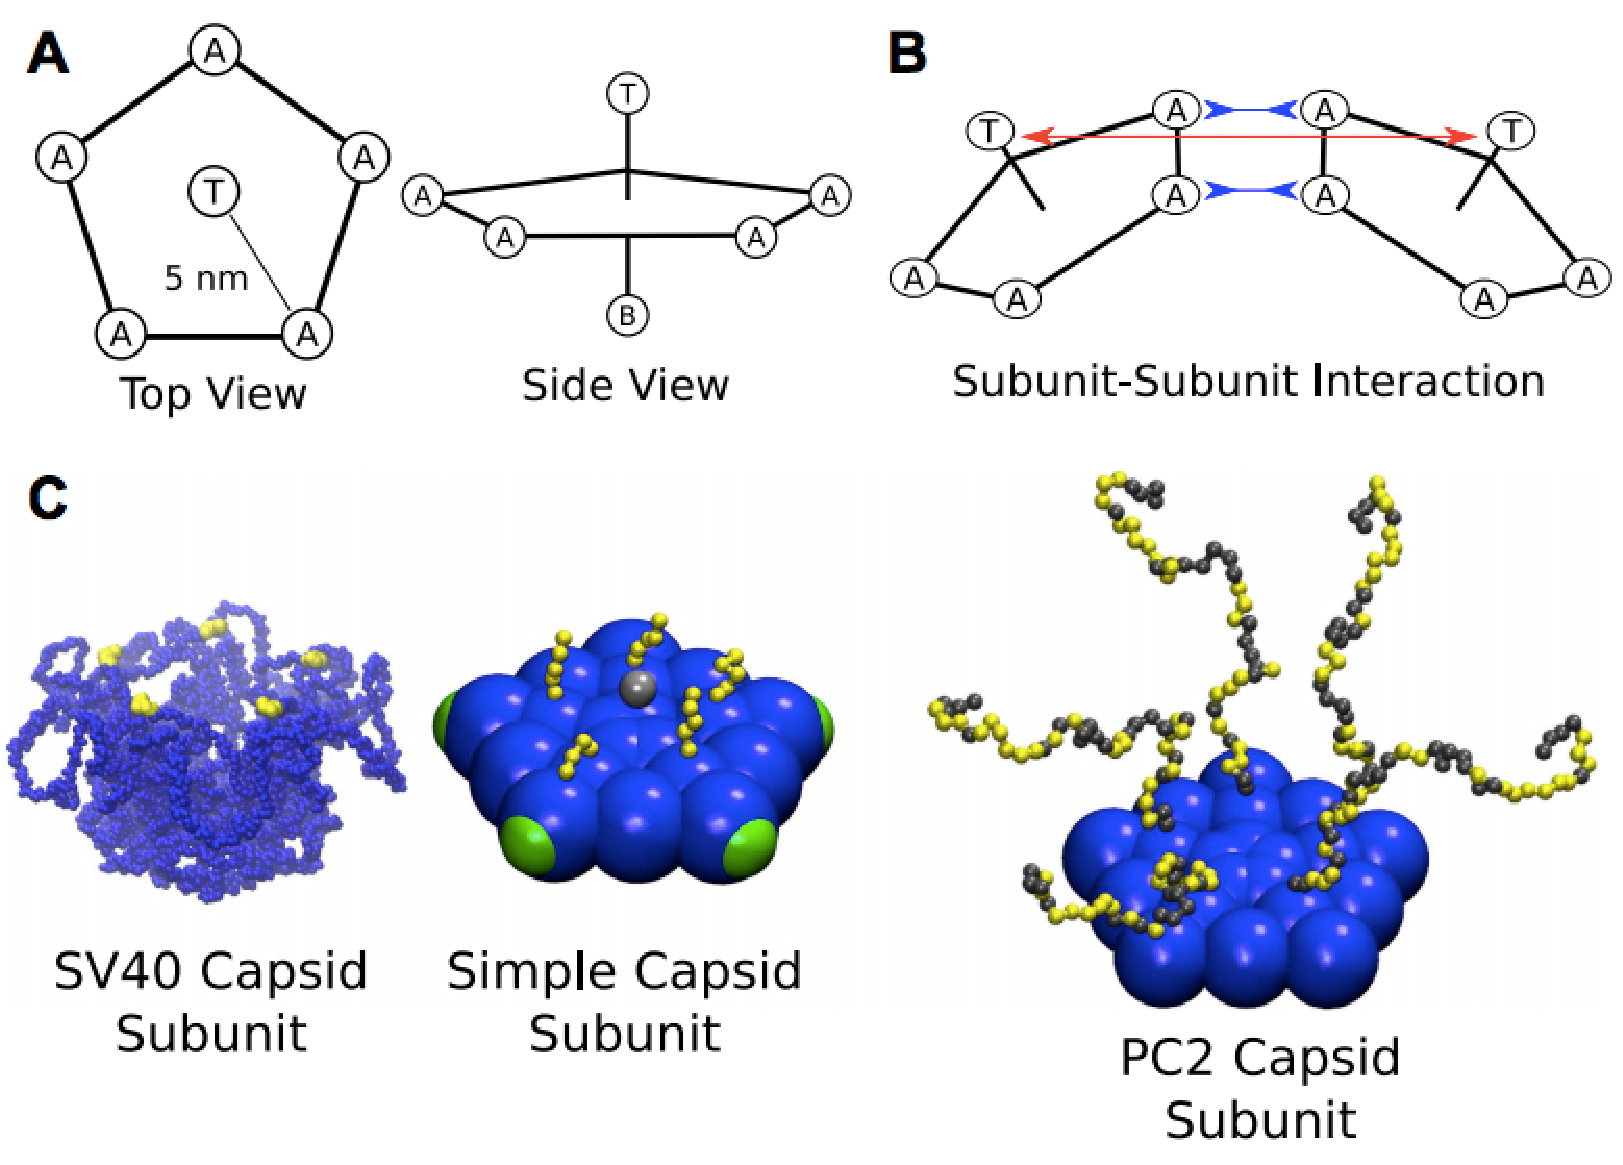
\includegraphics[width=0.4\textwidth]{capsid_face_diagram.pdf}
\end{center}

Recently Perlmutter et al. (2013) have used molecular dynamics to simulate the movement of components of a viral capsid and their interactions with the nucleic acid they are designed to contain. The steps in these simulations will be familiar to you from simulation of Langevin SDEs: in each step of the simulation the forces acting on each atom are calculated and used to update its position and momentum with added noise. To make the problem computationally tractable, the authors examined a dodecahedon capsid in which the faces are pentagons: the whole face is modeled by five ``atoms" arranged in a pentagon, each of which is attracted to like atoms on adjacent faces, and two ``atoms" above and below the face which repel one another with different strengths to position adjacent faces at an angle. Onto the interior faces are positioned strands of positive charges meant to represent the positive-charged residues that interact with the nucleic acid backbone. A ``nucleic acid" (chain of positive charges perhaps with secondary structure from hydrogen bonding) dropped into a solution of these capsid faces will tend to increase their local concentration enough to nucleate capsid assembly. The simulation can be repeated with nucleic acids of various sizes and secondary structures to study average time to assembly.\\

\begin{center}
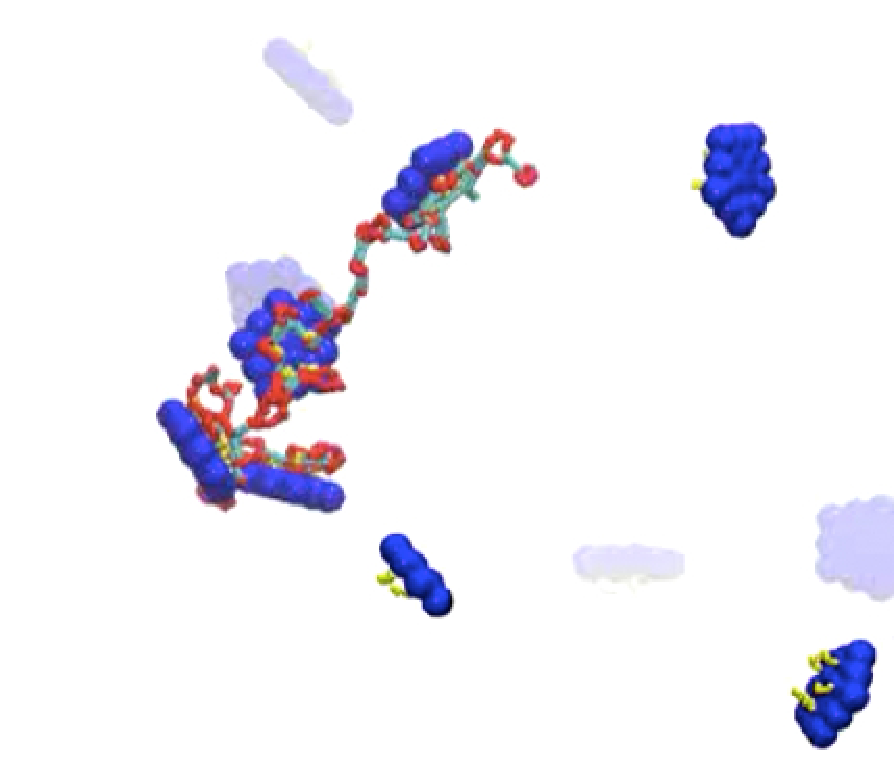
\includegraphics[width=0.3\textwidth]{assembly.pdf}
\end{center}

In such simulations, capsids will spontaneously assemble around a nucleic acid even if the NA's charge significantly exceeds that of the capsid faces. A more important determinant is the typical volume of the NA, determined both by its length and its folding pattern.\\

These simulations suggest another way in which capsids can be encouraged to assemble without unwanted interactions between host proteins: the NA acts to increase the local concentration of capsid faces and facilitates their interaction. HIV-1 also increases the local concentration of its capsid components via tethering even before its viral envelope has formed. The HIV-1 genome encodes a protein called Gag which is made up of many domains which will later be proteolytically cleaved during maturation. The N-terminal end of Gag (called MA) binds to the plasma membrane and to the HIV Env protein, the major components of the HIV envelope. The central region of Gag (called CA) will form the capsid, and the C-terminal end (called NC) will bind to the HIV genome to facilitate its inclusion in the virion. The interaction of Gag with the plasma membrane ensures its enriched concentration there so that nonspecific binding of CA with host proteins is less likely. (Interestingly the binding between CA domains at this stage is different from the interaction in the mature capsid, permitting formation of a dome rather than a cone.) Co-expression of these proteins in the long polypeptide Gag also ensures a fixed stoichiometry within the virion.

\begin{center}
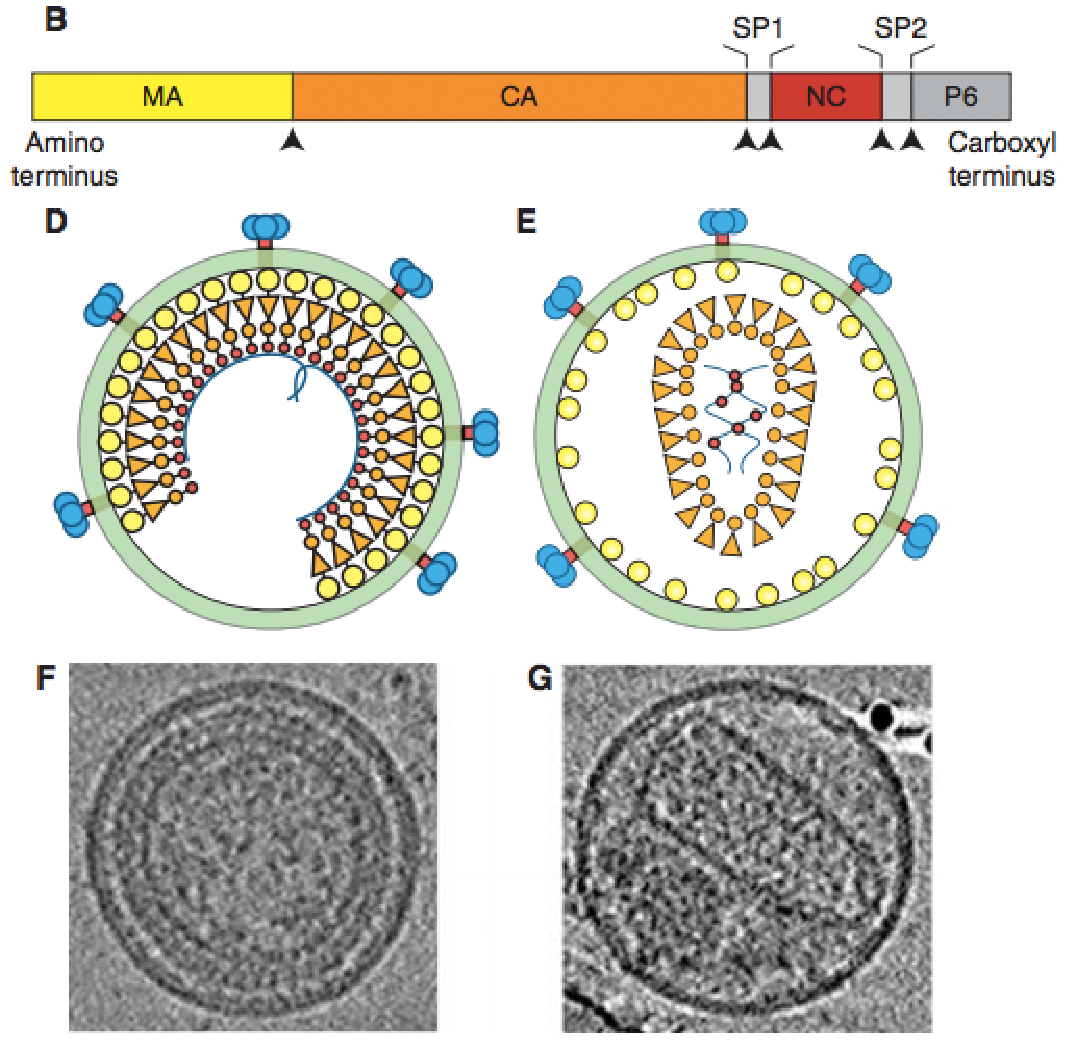
\includegraphics[width=0.7\textwidth]{hiv.pdf}
\end{center}


\section*{Influenza A}

Influenza A, the most virulent form of flu, is a single-stranded RNA virus which encodes its genome on eight separate RNA molecules. It lacks a tight capsid but rather encloses its genome and other proteins within a viral envelope made of viral proteins and the host's plasma membrane. To be effective, a virion must be packaged with one of each of these RNAs: there appears to be no room for an extra copy of any. Specific ``packaging sequences" have been identified on the viral RNAs without which most virions have an incorrect complement of RNAs.

\begin{center}
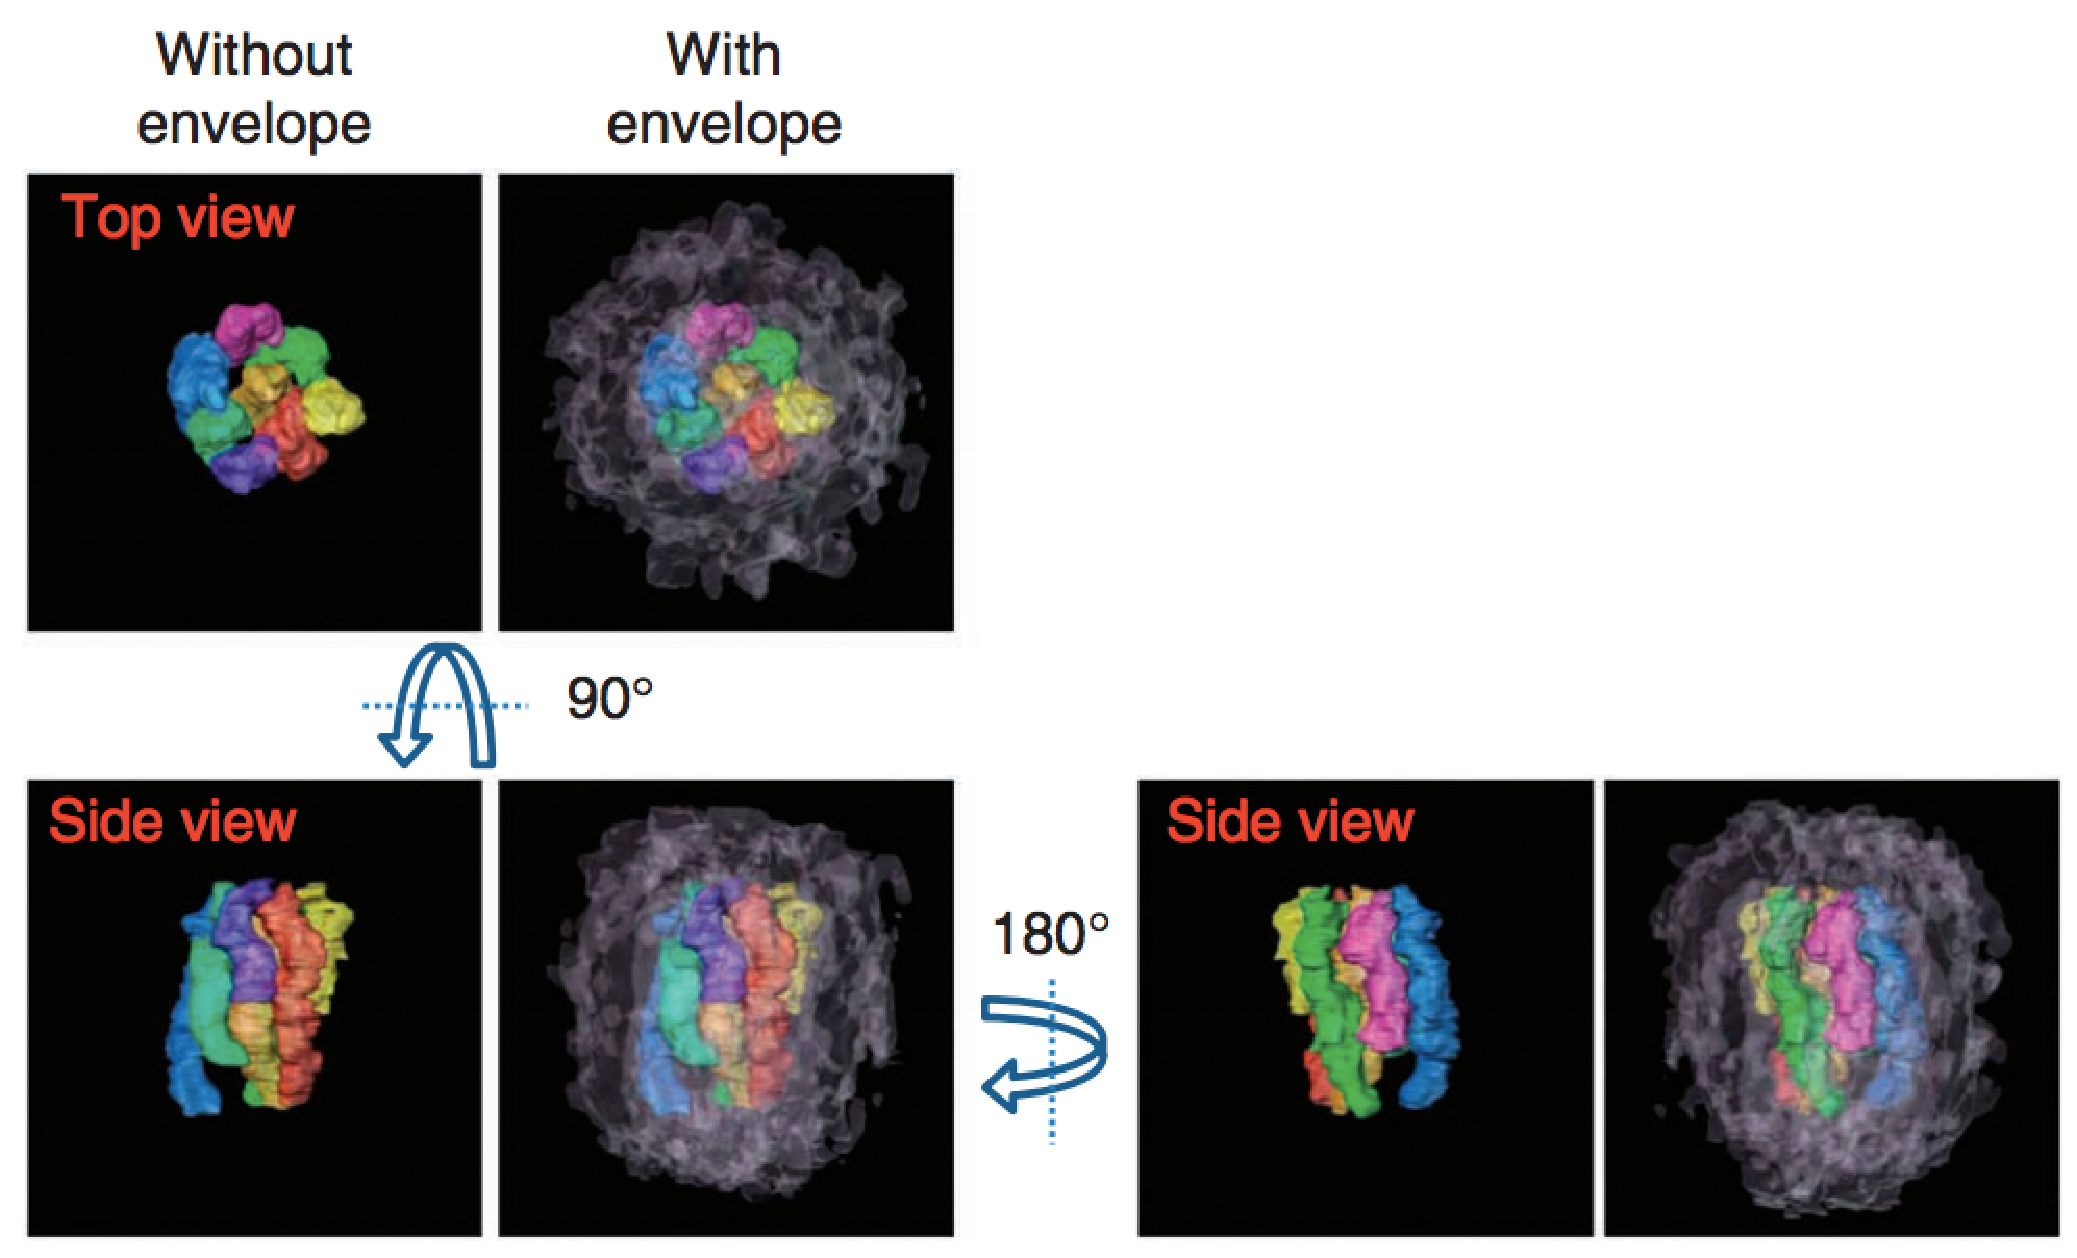
\includegraphics[width=0.5\textwidth]{noda.pdf}
\end{center}

Consider two alternative hypotheses for how these packaging sequences could work. In the first, packaging sequences help RNAs to bind to one another (either directly or via RNA-protein interactions). Carefully orchestrated interactions would bring exactly the right set of eight RNAs together under this theory. I will bet green cash that this is the approach any of us would take if asked to design a self-assembling virion. However, there is no evidence for spatial order of the RNAs within the envelope. An alternative hypothesis is that packaging sequences introduce repulsion between like RNAs. Repulsion could be thought of simply as an absence of interactions possible between other sequences. (Steric hindrance and electrostatic based on positioning of packaging sequences on loops is also imaginable but not discussed below.)Unlike the first model, each RNA's self-repulsion system could evolve independently under this theory and there would be no constraints on co-evolution of e.g. the packaging sequences between RNAs, and no requirement for spatial order. On the other hand, one of the advantages of the specific positive interaction model is that it explains why host RNAs are rarely included in the virion by mistake.

\begin{center}
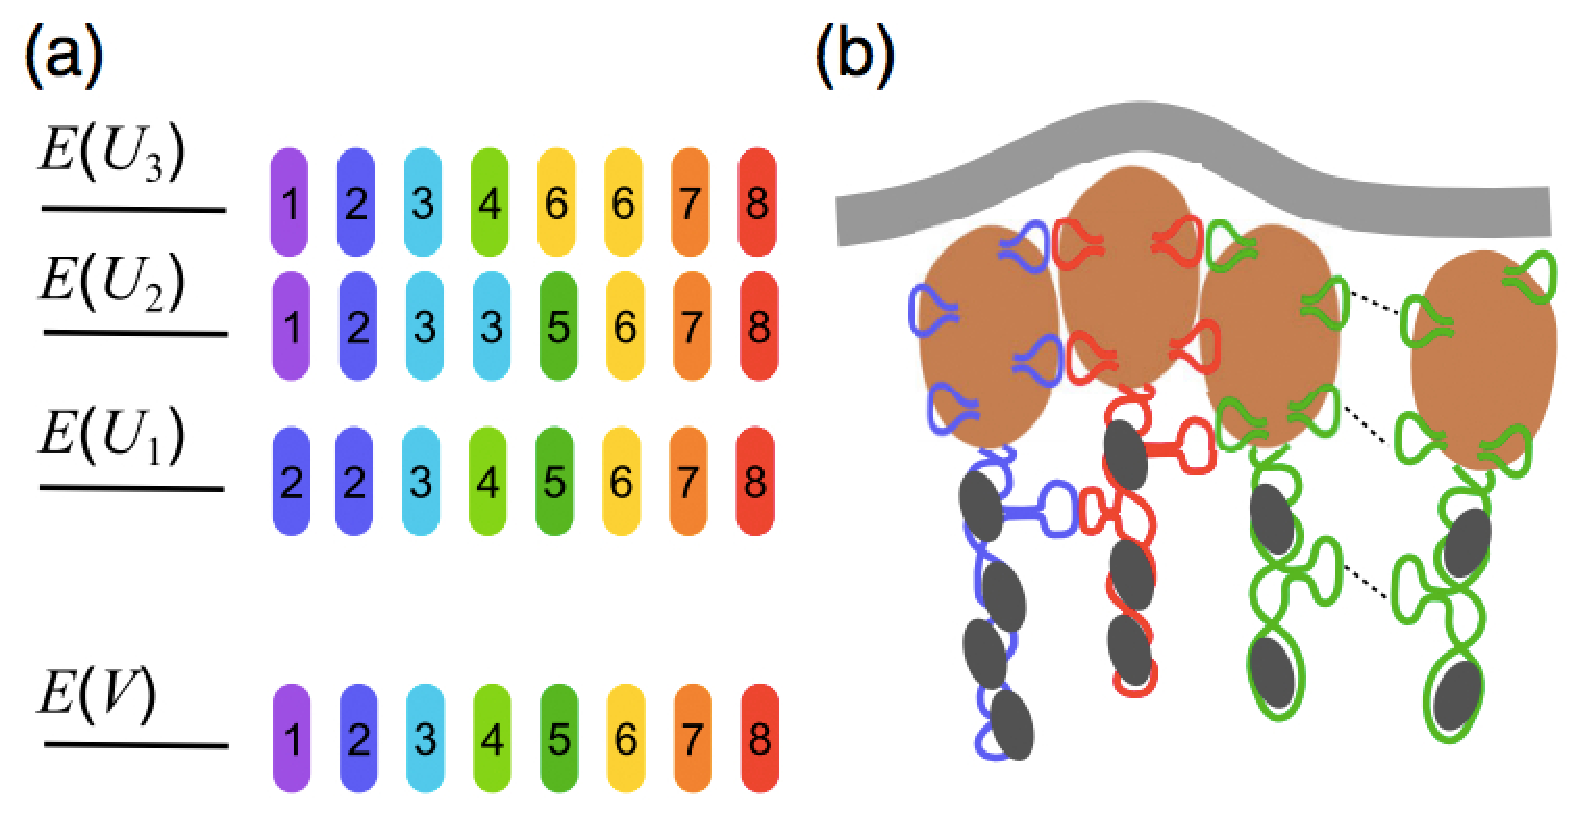
\includegraphics[width=0.5\textwidth]{venev1.pdf}
\end{center}

The plausibility of this model was investigated by Venev and Zeldovich (2013) using an \textit{in silico} evolution approach. They envision an interaction energy $E$ which depends on the number of each type of RNA that can be included in the virion. They assume that the envelope does not have room for extra RNAs and that eight RNAs are always included; they also assume that only the simplest mistakes -- leaving out one RNA and including two of another -- occur, so that there are 56 possible errors and one correct combination\footnote{This assumption may seem arbitrary but is reasonably justified by experimental analysis of single virions, c.f. Noda et al. (2012) and Chou et al. (2012).}. The combination of RNAs in an envelope can be described by a packaging index: for example, $V=(1,1,1,1,1,1,1,1)$ represents correct packaging and $U_{12}=(0,2,1,1,1,1,1,1)$ one possible error. The interaction energy also depends on the spatial position $k$ in which these RNAs happen to find themselves. The probability of correct binding is given by a Boltzmann factor:
\[ \Pi = \frac{\sum_{k} e^{-\beta E(V,k)}}{\sum_{k} e^{-\beta E(V,k)} + \sum_{k,i,j} e^{-\beta E(U_{ij},k)}} \]
The interaction energies depend on the sequences of the packaging loops, which are allowed to evolve in the simulation and assumed to depend only on Watson-Crick base pairing.

\begin{center}
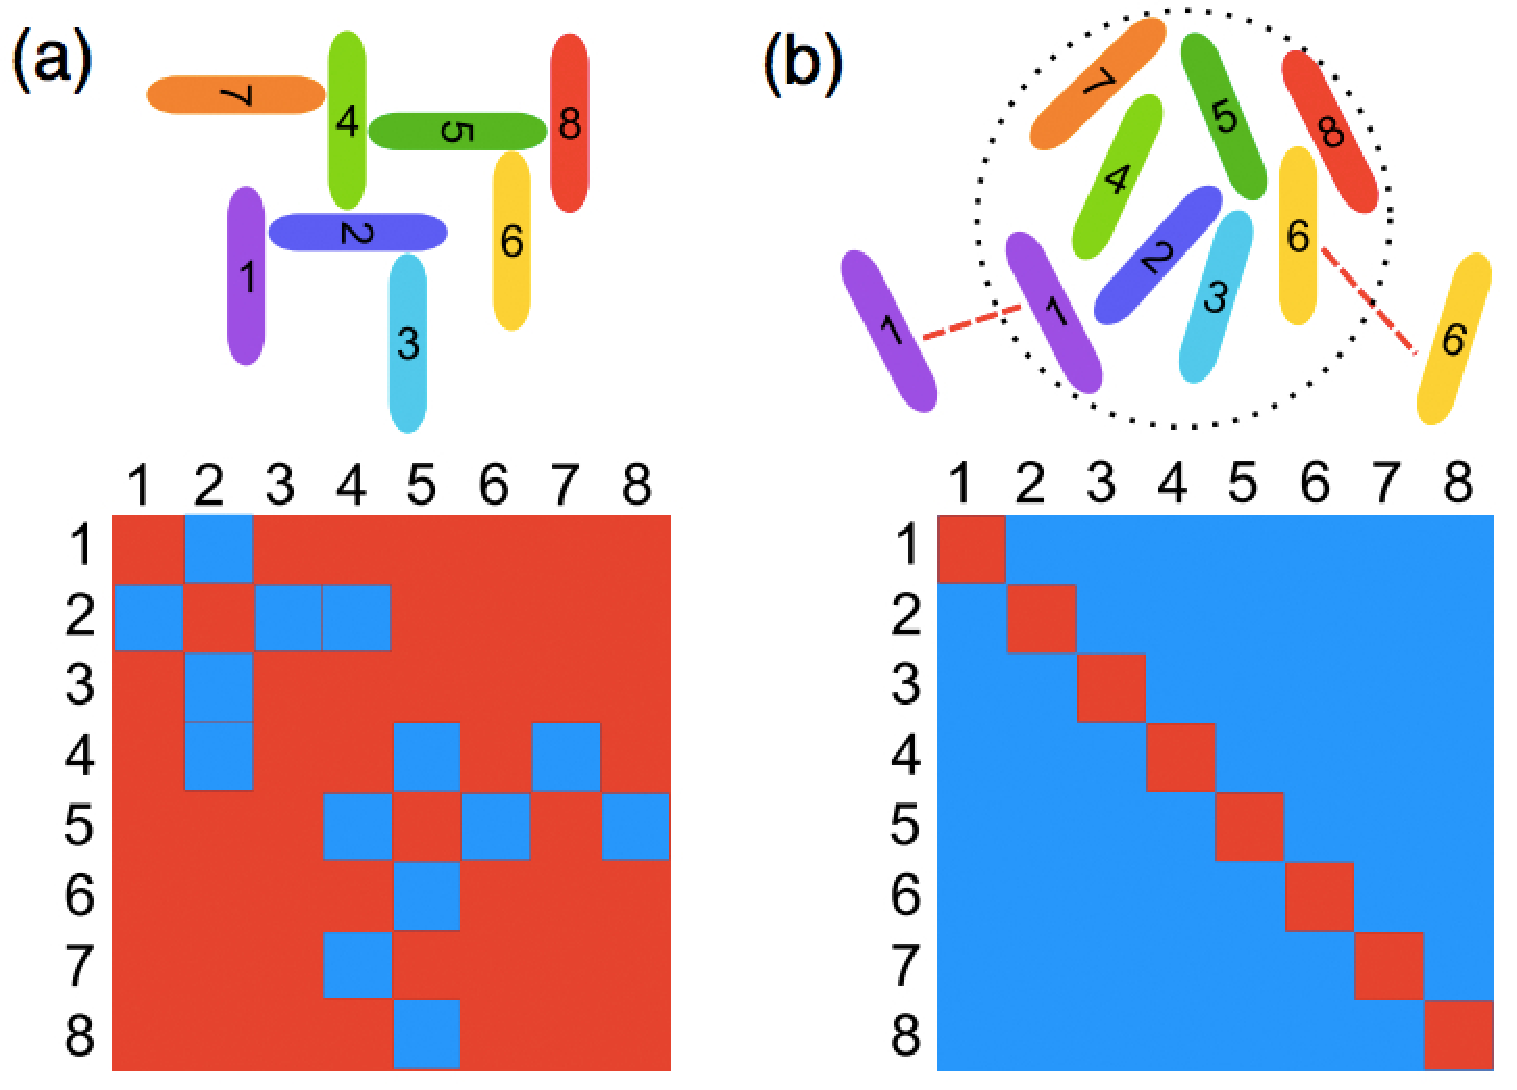
\includegraphics[width=0.5\textwidth]{venev2.pdf}
\end{center}

Venev and Zeldovich reasoned that if the first model were correct, at the end of the simulation they could expect to see strong positive interactions between certain pairs of RNAs (which must form a network connecting all eight RNAs) and relatively weak interactions between all others. However, if the second model were correct, all but the self-interactions would be relatively strong. The latter best describes what they observed in sequences that were evolved to maximize $\Pi$. The maximum value for $\Pi$ which they obtained by this method was 0.35, on par with the $\approx$50\% correct virion assembly rate estimated experimentally via FISH and electron tomography (Chou et al., 2012 and Noda et al., 2012).

\begin{center}
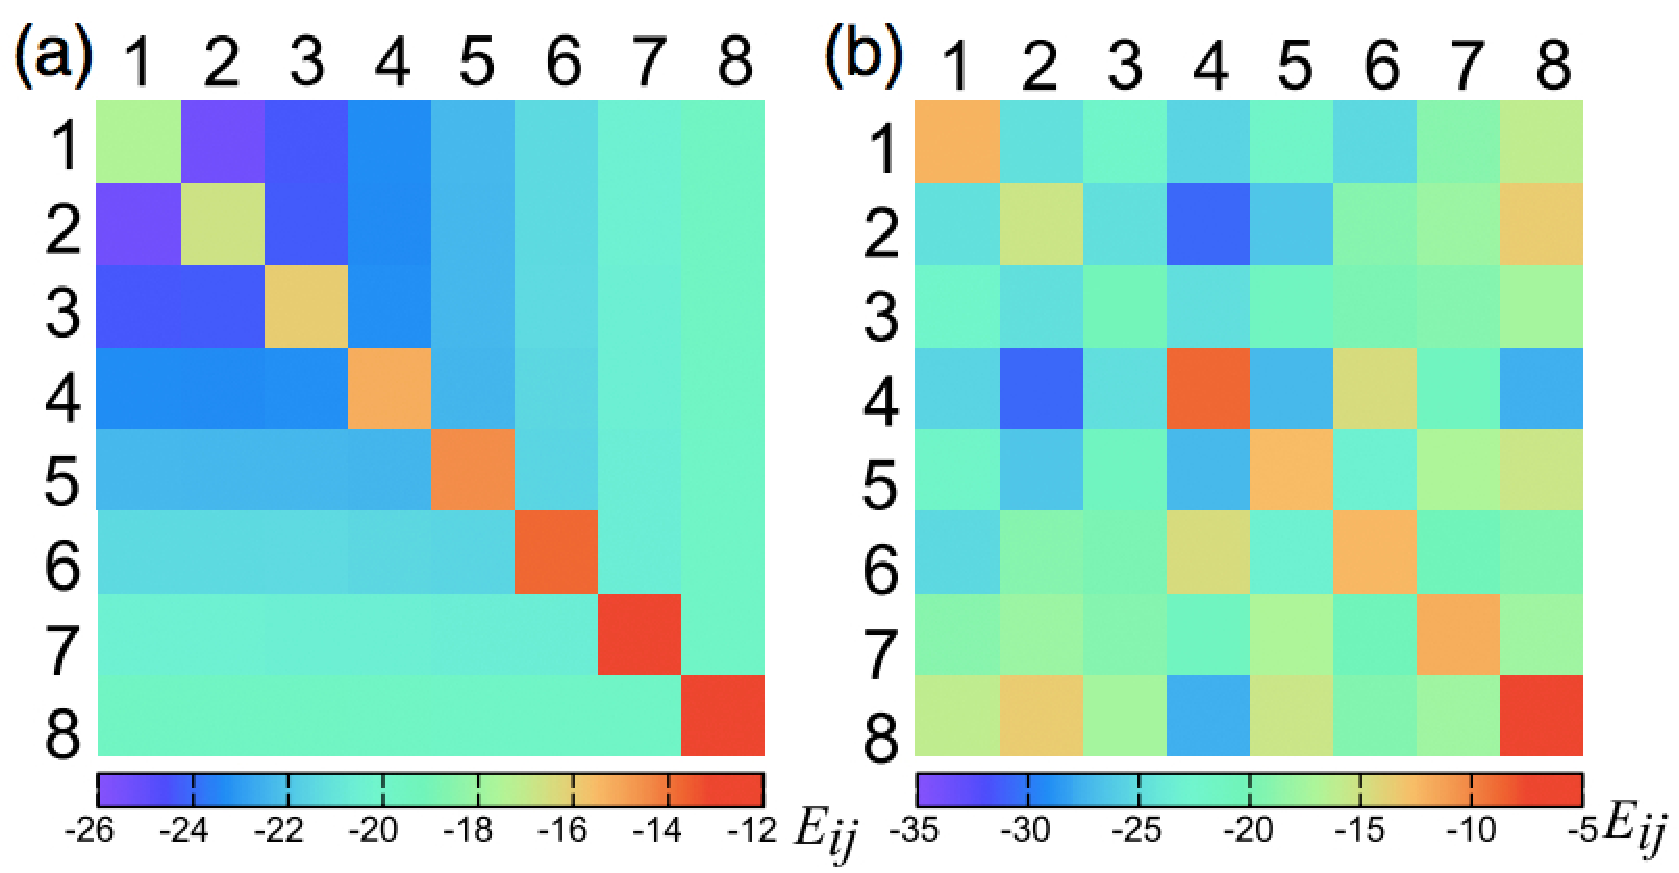
\includegraphics[width=0.5\textwidth]{venev3.pdf}
\end{center}

\section*{Self-assembly of genomes}

Annaluru et al. (2014) recently reported the synthesis of a complete chromosome in \textit{S. cerevisiae}, the first step in a project to create the first synthetic eukaryotic genome (Sc2.0). Reconstructing a genome provides the opportunity to test many theories concerning its function. For example, it is known that roughly 5000 of \textit{S. cerevisiae}'s 6000 genes are non-essential when deleted alone, and much is also known of epistasis in gene pairs; however, it is not known what complement of genes is minimal for survival. The synthetic genome will flank open reading frames with loxP sites: recombinants which have had the opportunity to remove genes (or rearrange them) can be isolated after recombinase activity to assess which genes are essential. One stop codon will also be completely absent in open reading frames of this synthetic genome, so that synthetic tRNAs with a complementary anticodon can be used to label a protein of choice with a non-canonical amino acid. Alterations to the genome have also been used to confirm or refute experimental predictions involving the sufficiency of telomeric repeats, the role of tRNA genes in cohesin recruitment, removal of repetitive sequences that were once hotspots for genomic rearrangements, and reduction of introns (where this does not interfere with fitness). Ultimately, the construction of synthetic genomes could be used to produce species which grow optimally under defined conditions.

\begin{center}
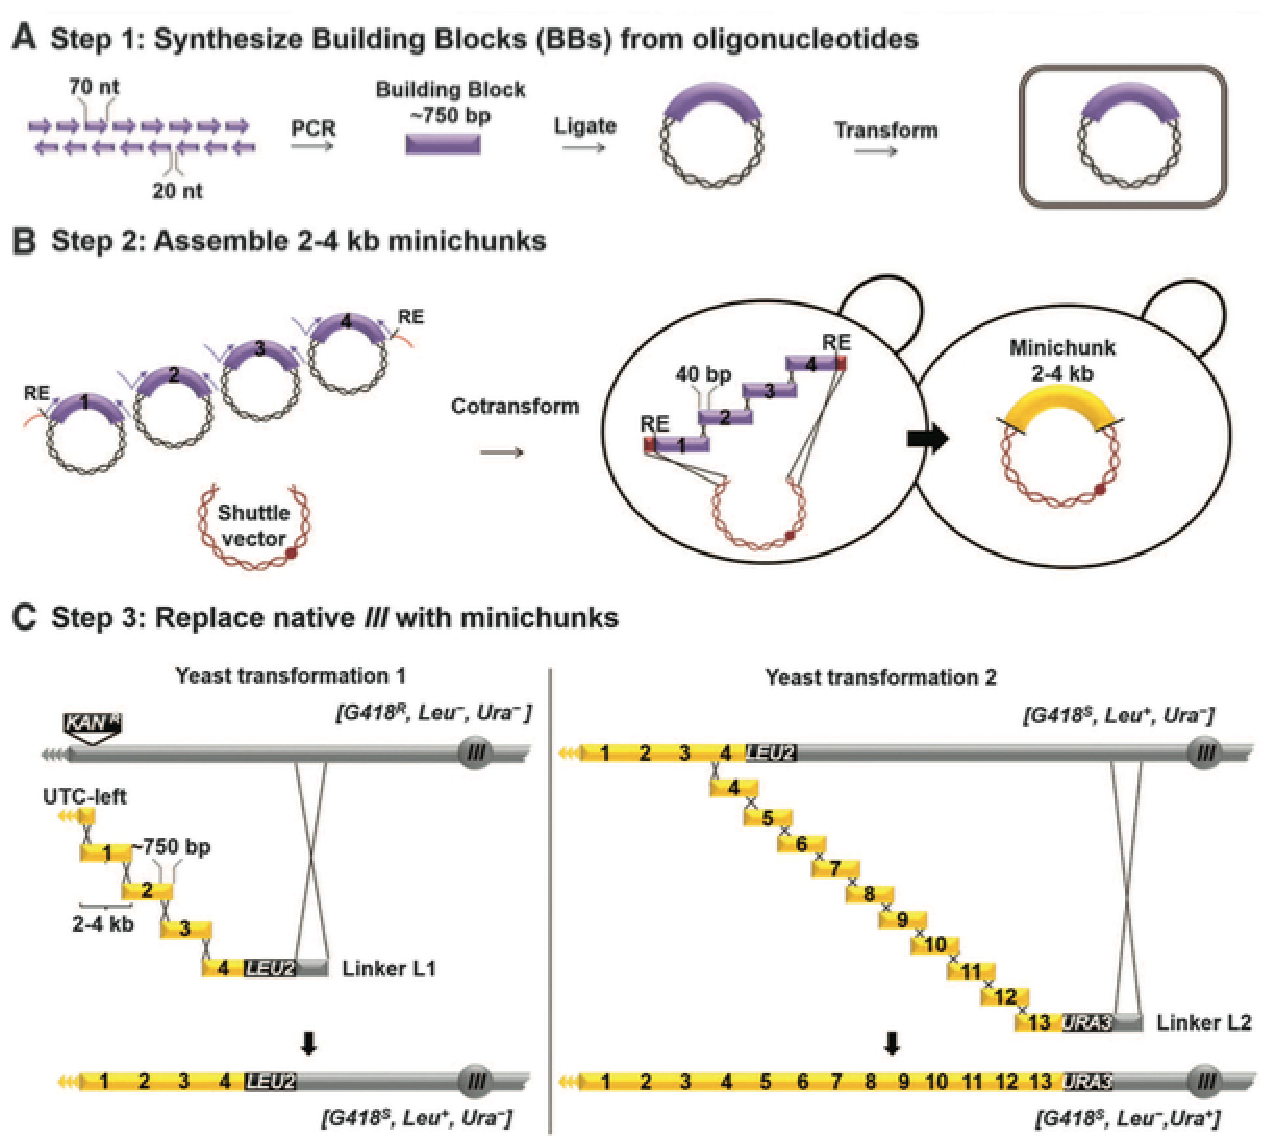
\includegraphics[width=0.5\textwidth]{annaluru.pdf}
\end{center}

Construction of the synthetic chromosome begins with 750 bp blocks constructed by hybridizing overlapping 70 nt oligonucleotides and employing PCR to assemble these into a complete double-stranded DNA ``building block" (Stemmer et al., 1995). Fusion PCR is then used to assemble 3-4 building blocks into an approx. 3 kb ``mini-chunk." Multiple minichunks which overlap one another are cotransformed into yeast, where they integrate with the genome and one another by homologous recombination. (If the sequence of any mini-chunk makes the host inviable, the transformation fails and a new sequence can be attempted.) With this approach the authors were able to walk along the chromosome until it had been fully replaced with synthetic sequence. This synthesis strategy mirrors the approach used by the Venter Institute to synthesize and replace genomes in \textit{Mycoplasma} (Gibson et al., 2010).

\section*{DNA origami}

\begin{center}
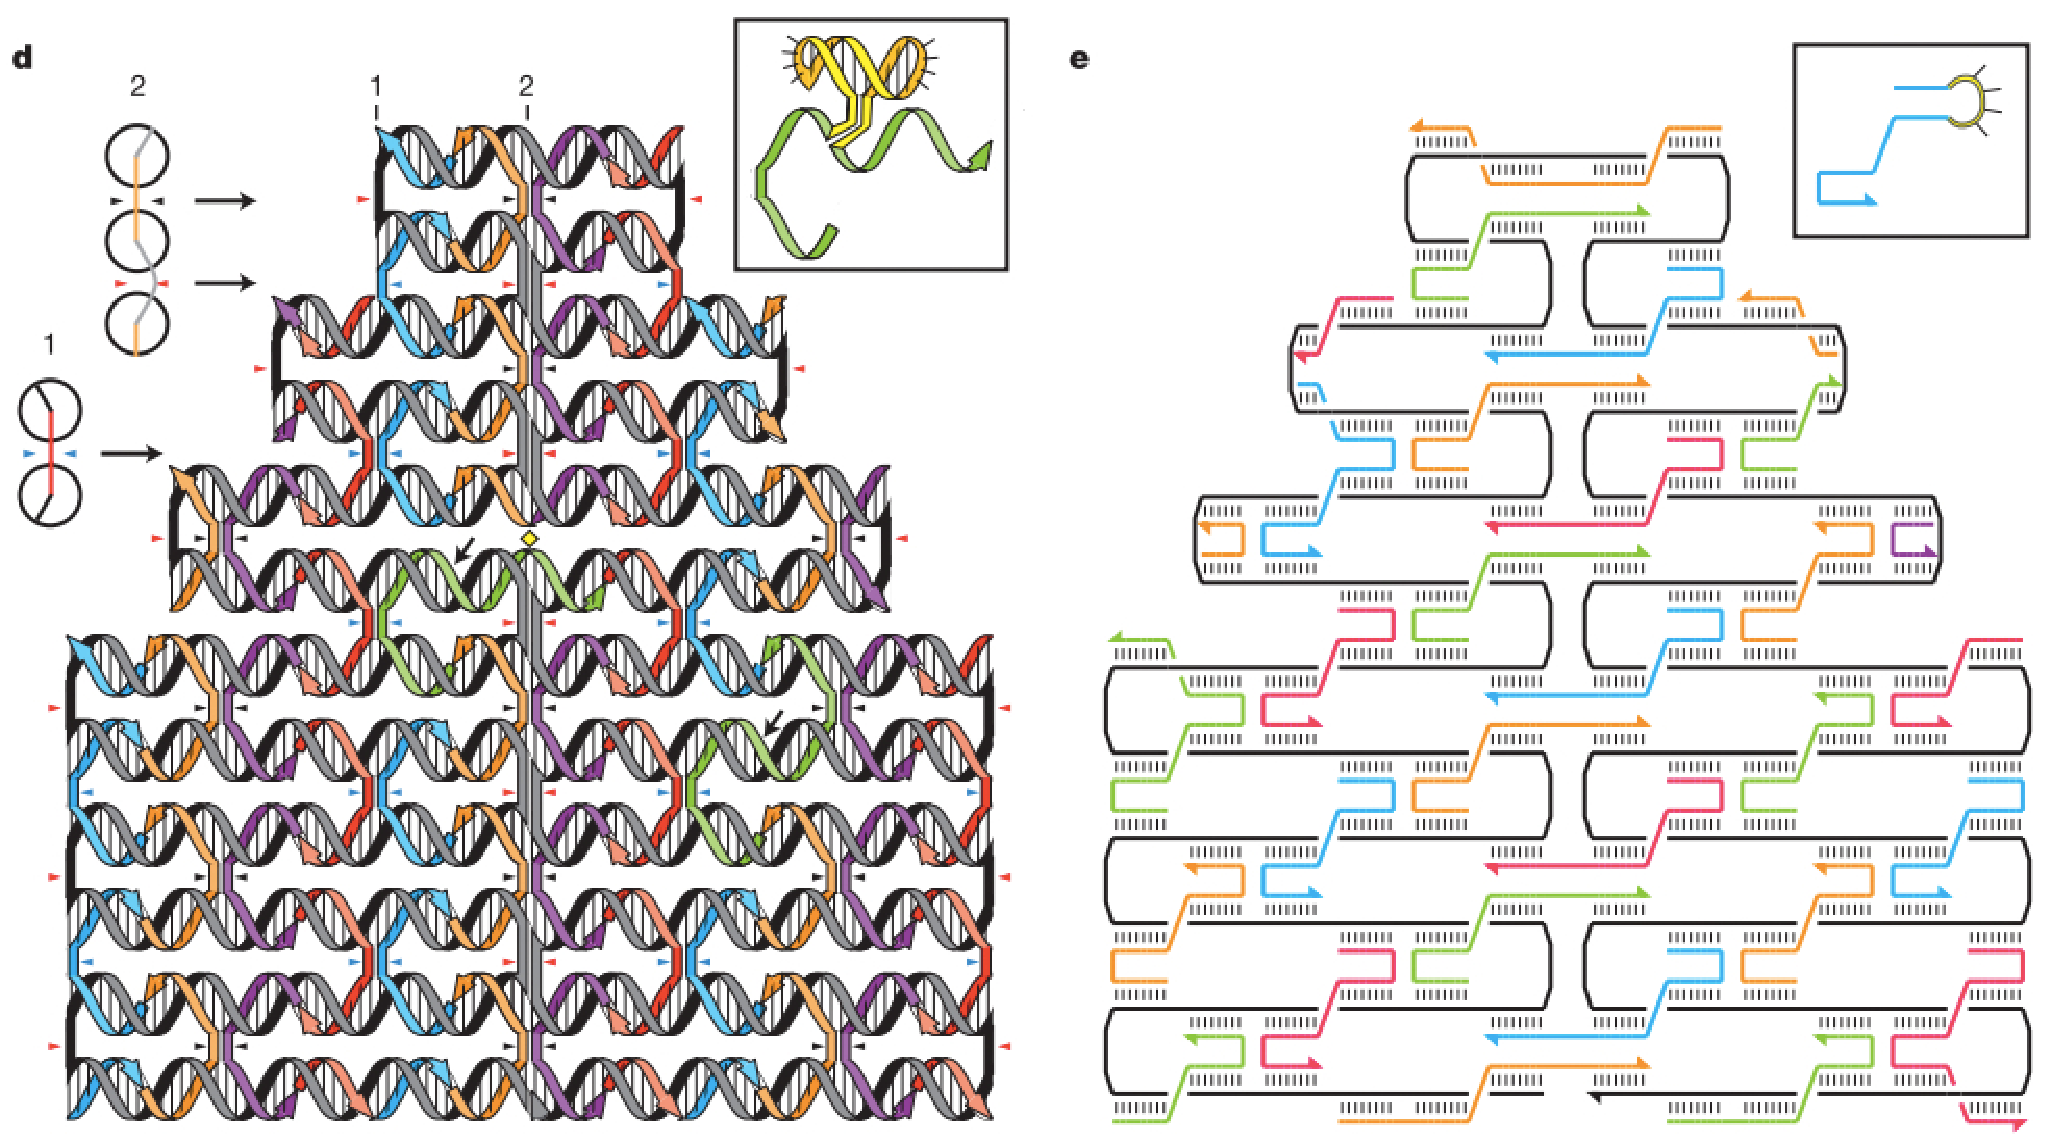
\includegraphics[width=0.5\textwidth]{rothemund1.pdf}
\end{center}

Computational design of nucleic acids which partially hybridize to form arbitrary shapes has been continually improving since Paul Rothemund introduced the technique in 2006. Rothemund's method used the 7kb single-stranded DNA genome of the phage M13mp18 as a ``scaffold" which was forced to bend by sequence-specific hybridization to smaller DNA ``staples" that bound to two different genomic regions to pull them physically together. Heating the combination of DNAs together and allowing them to very slowly cool and anneal produces the arbitrary shapes, which can be visualized by EM.

\begin{center}
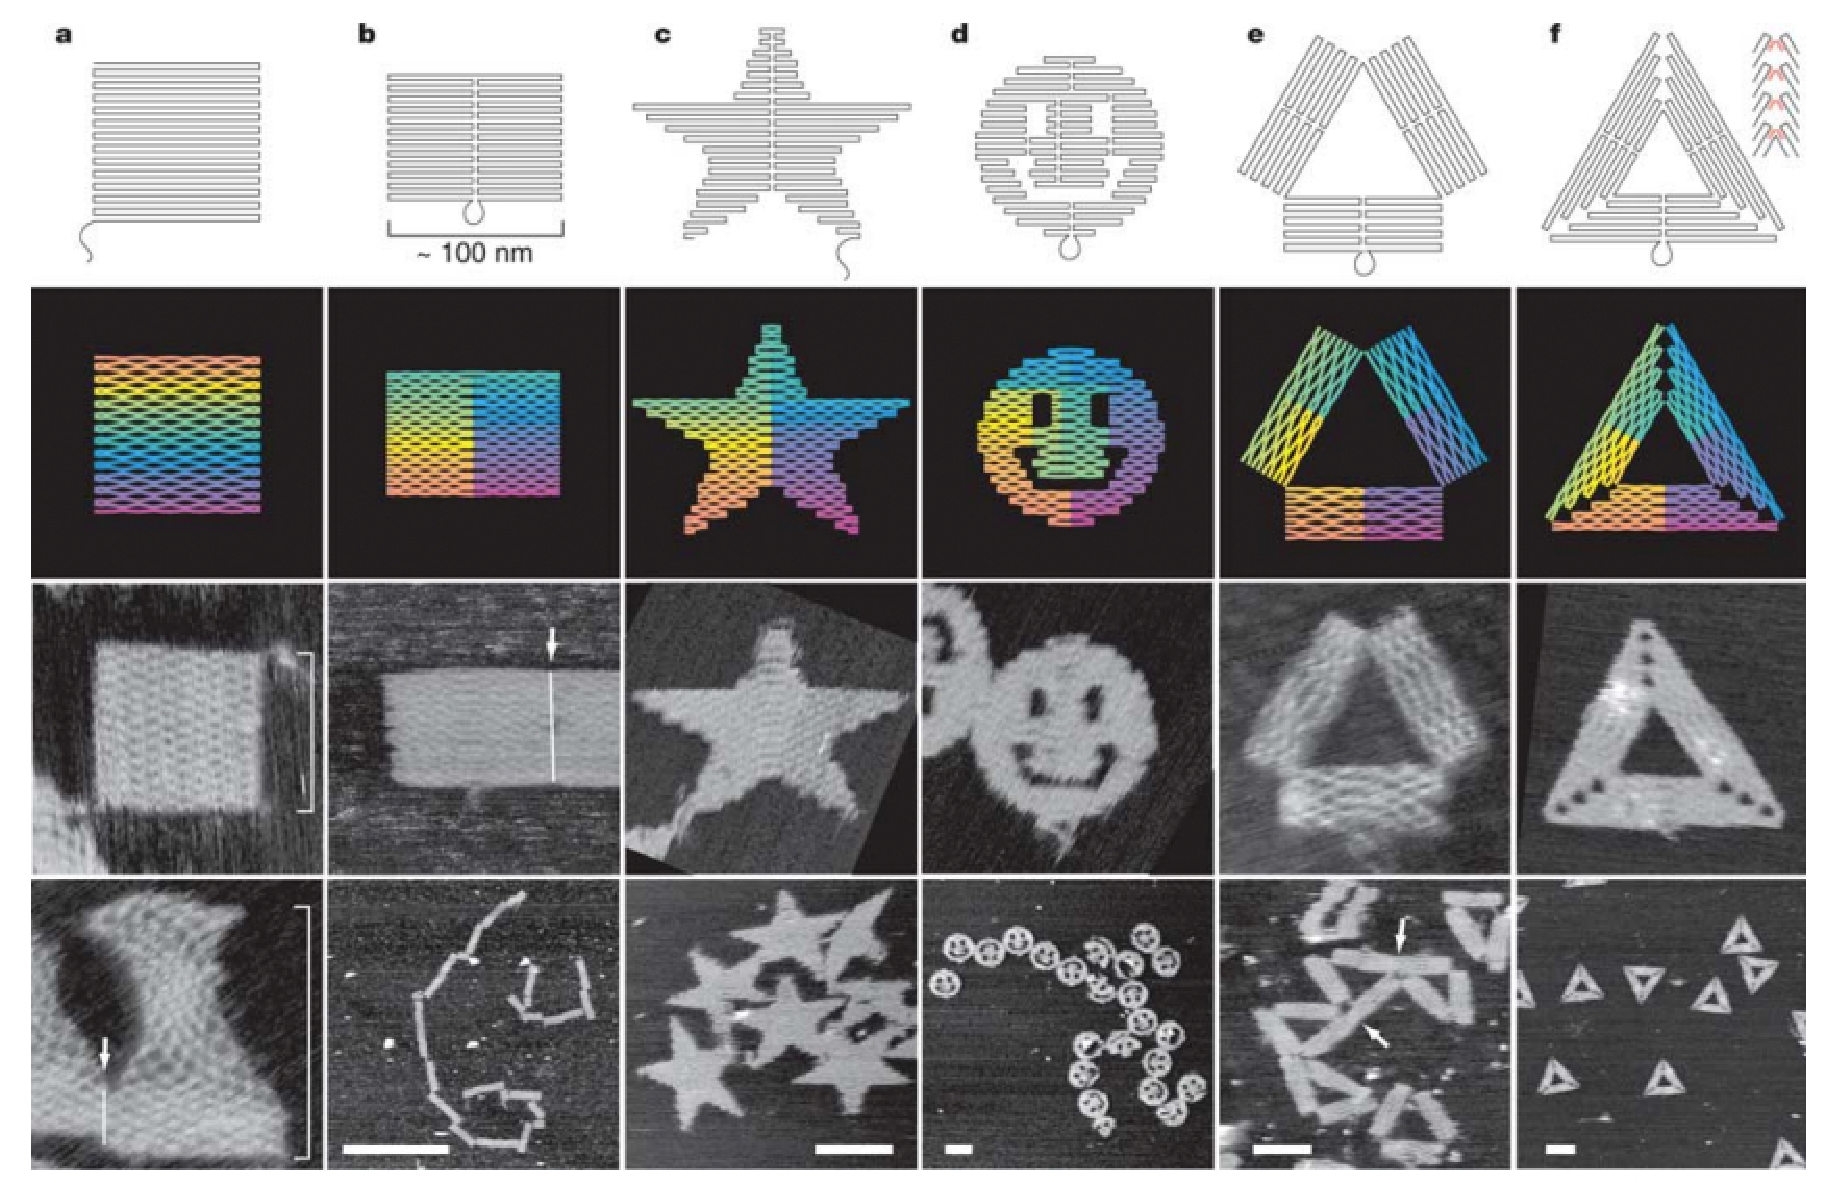
\includegraphics[width=0.5\textwidth]{rothemund2.pdf}
\end{center}

Just as in PCR primer design, algorithmic design of hybridization sequences reduces the probability of undesired binding events. Full control over the sequence can be had by swapping the viral genome scaffold for fully-synthetic sequences; many shapes can be constructed from a small number of appropriately-chosen sequences (Wei et al., 2010). The error rate can also be tuned by choosing an appropriate stoichiometry between the nucleic acids, which does not necessarily reflect the stoichiometry in the correct structure but may instead be chosen to disfavor incorrect structures from forming (Murugan et al., 2015).\\

The shapes chosen to test these sequence-selecting algorithms are often whimsical to demonstrate the versatility of the method. Of course three dimensional shapes can be constructed by a similar approach (Ke et al., 2012), including some which execute assembly reactions in a specific order (Sadowski et al., 2014).\\

Recently DNA origami has also been employed to create ``molds" in which metal deposits can be nucleated to form specific shapes (Sun et al., 2014). Boxes made from DNA have also been caused to execute logic functions with the goal of delivering their ``contents" only under specific conditions (Amir et al., 2014).

\begin{center}
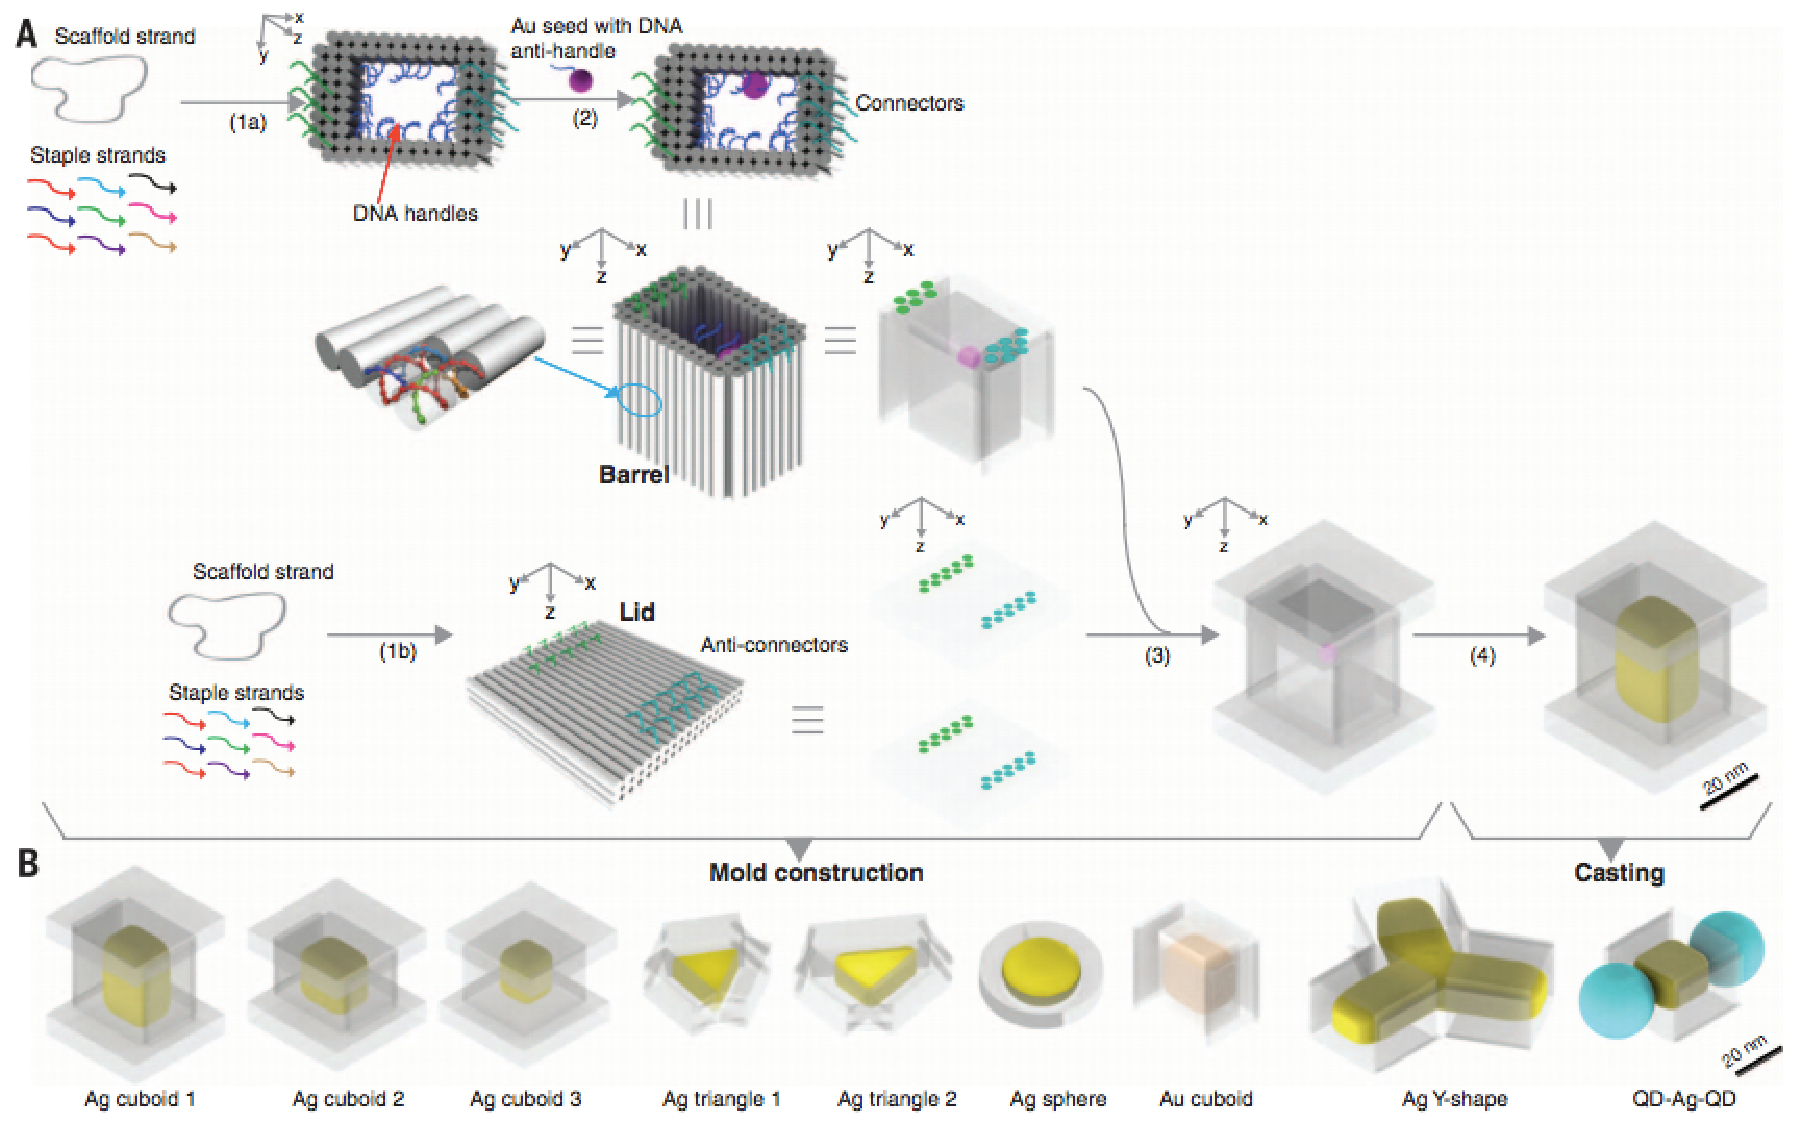
\includegraphics[width=0.5\textwidth]{mold.pdf}
\end{center}

\section*{Self-replication}

In the majority of this lecture, we have treated self-assembly as a spontaneous process involving only interactions between the building blocks during assembly. Though this approach is used often in both natural and synthetic biological systems, in many cases assembly requires a more direct agent. If that agent is an already-assembled entity of the same type, the process is still considered a form of self-assembly but is more likely to be referred to as self-replication.\\

The ``RNA world" hypothesis holds that nucleic acids once served as both genetic material and catalytic agents (a function they continue to perform today, e.g., at the heart of the ribosome). One possibility for the origin of life is that a single nucleic acid became capable of folding in such a way that it could replicate itself (or at least, copies of itself). Alternatively, a small number of nucleic acids may form a cooperative network which favors the replication of all components. It is theoretically possible through artificial selection or experimental evolution to produce an RNA which is capable of templated nucleotide polymerization. Since binding free nucleotides could be imagined to be an important function for self-replicating RNAs, an interesting first-pass is to select just for e.g. ability to bind GTP, an experiment which has already been performed using an exhaustive covering of the sequence space for 24-nt RNAs (Jim\'{e}nez et al., 2014). Longer RNAs capable of extending a dsRNA overhang up to their own length have been evolved through directed evolution (see e.g. Attwater et al., 2013) and can function under imperfect conditions such as within ice. Important functions such as priming and loss of the fully double-stranded state for folding into the functional state prevent these RNAs from being fully capable of self-replication, however.\\

The general principle that a parent entity may serve as a template over which a new one could be assembled from its constituent parts has also been studied in model systems that permit simulation and functional analysis. A model based on a catalytic pair of structures formed from interacting spheres can be modeled by an approach similar to molecular dynamics (Zeravcic and Brenner, 2014). These toy models reveal that even a relatively simple system can be capable of self-replication.



\end{document}